\chapter{Fuentes de campo magnético}
\section{Campo de una carga en movimiento}
Comenzaremos con lo fundamental: el campo magnético de una sola carga puntual $q$ que se mueve con velocidad constante $\vec{v}$. Los experimentos demuestran que la magnitud de $\vec{B}$ es proporcional a $|q|$ y a $1/r^2$, pero su dirección \textit{no} es a lo largo de de la línea que va desde el punto de fuente al punto de campo. En vez de ello, $\vec{B}$ es perpendicular al plano que contiene esta línea y al vector velocidad, de la partícula, $\vec{v}$. Además, la magnitud $\vec{B}$ del campo también es proporcional a la rapidez $\vec{v}$ de la partícula y al seno del ángulo $\phi$. Así, la magnitud del campo magnético en el punto $P$ está dada por
\begin{equation}\label{28.1}
B=\frac{\mu_0}{4\pi}\frac{|q|v\sin\phi}{r^2}
\end{equation}
donde $\mu_0/4\pi$ es una constante de proporcionalidad.
En forma vectorial
\begin{equation}\marginnote{C. magnético de una carga puntual con velocidad constante}
\boxed{\vec{B}=\frac{\mu_0}{4\pi}\frac{q\vec{v}\times\hat{r}}{r^2}}
\end{equation}
\textbf{Nota}: Las partículas con carga que constituyen una corriente en un alambre aceleran en los puntos en que éste se dobla y la dirección de $\vec{v}$ cambia. Pero como la magnitud $v_d$ de la velocidad de deriva en un conductor por lo general es muy pequeña, la aceleración $v_d^2/r$ también lo es, por lo que pueden ignorarse los efectos de la aceleración.

La unidad en el SI de $B$ es un \textbf{tesla} [1T].

En unidades del SI, el valor numérico de $\mu_0$ es exactamente $4\pi\times 10^{-7}$
\section{Campo magnético de un elemento de corriente}
\textbf{Principio de superposición de campos magnéticos}:  El campo magnético total generado por varias cargas en movimiento es la suma vectorial de los campos generados por las cargas individuales.

\textit{Cálculo del campo magnético ocasionado por un segmento corto $d\vec{l}$ de un conductor que transporta corriente}:

El volumen del segmento es $A dl$, donde $A$ es el área de la sección transversal del conductor. Si hay $n$ partículas con carga en movimiento por unidad de volumen, cada una con una carga $q$, la carga total $dQ$ que se mueve en el segmento es $$dQ=nqAdl$$ Las cargas en movimiento en este segmento son equivalentes a una sola carga $dQ$
que viaja con una velocidad igual a la velocidad de \textit{deriva} $\vec{v}_d$. (Los campos magnéticos debidos a los movimientos al azar de las cargas, en promedio, se cancelarán en cada punto.) De ec. \ref{28.1}, la magnitud del campo resultante $d\vec{B}$ en cualquier punto $P$ es
\begin{equation}\label{28.5}
dB=\frac{\mu_0}{4\pi}\frac{|dQ|v_d\sin\phi}{r^2}=\frac{\mu_0}{4\pi}\frac{n|q|v_dAdl\sin\phi}{r^2}=\frac{\mu_o}{4\pi}\frac{Idl\sin\phi}{r^2}
\end{equation} 
porque de ec (25.2), $n|q|v_dA$ es igual a la corriente $I$ en el elemento.

En su forma vectorial
\begin{equation}\label{28.6}\marginnote{C. magnético de un elemento de corriente}
\boxed{d\vec{B}=\frac{\mu_0}{4\pi}\frac{Id\vec{l}\times\hat{r}}{r^2}}
\end{equation}
donde $d\vec{l}$ es un vector con longitus $dl$, en la misma dirección que la corriente del coductor.
 
Las ecuaciónes \ref{28.5} y \ref{28.6} constituyen la \textbf{ley de Biot y Savat}. Esta ley se utiliza para encontrar el campo magnético total $B$ debido a la corriente en un circuito completo en cualquier punto en el espacio.
\section{Campo magnético de un conductor que transporta corriente}
\begin{figure}[h]
\centering
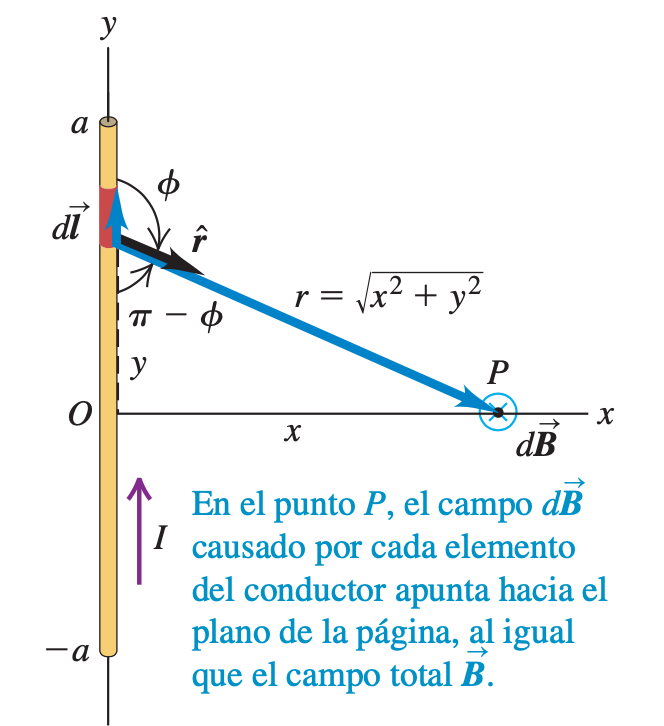
\includegraphics[scale=0.6]{fig/image1}
\caption{Campo magnético producido por un conductor recto portador de corriente de longitud infinita.}
\label{fig:28.5}
\end{figure}
Usando la ley de Biot y Savat, ecuación \ref{28.6}, y haciendo los cálculos correspondientes, se tiene que $B$ debe tener la misma magnitud en todos los puntos de un círculo con centro en el conductor y que yace en un plano perpendicular a él, y la dirección de $B$ debe ser tangente a todo ese círculo. Así, 
\begin{equation}\label{28.9}\marginnote{C. magnético cerca de un conductor largo y recto portador de corriente}
\boxed{\vec{B}=\frac{\mu_0I}{2\pi r}\hat{\phi}}
\end{equation}
\textbf{Observaciones:}
\begin{enumerate}
\item Las líneas de campo magnético circundan la corriente que actúa como su fuente.
\item Las líneas del campo magnético forman espiras cerradas y \textit{nunca} tienen extremos, sin importar la forma del conductor portador de corriente que genera el campo. Ésta es una consecuencia de la ley de Gauss para el magnetismo, que plantea que el flujo magnético total a través de cualquier superficie cerrada siem- pre es igual a cero:
\begin{equation}\label{28.10}
\oint\vec{B}\cdot d\vec{A}=0
\end{equation}
Esto implica que no hay cargas magnéticas aisladas ni monopolos magnéticos. \textbf{Cualquier línea de campo magnético que entre a una superficie cerrada debe salir de ella}.
\end{enumerate}
\section{Fuerza entre alambres paralelos}
\begin{figure}[h]\label{fig2}
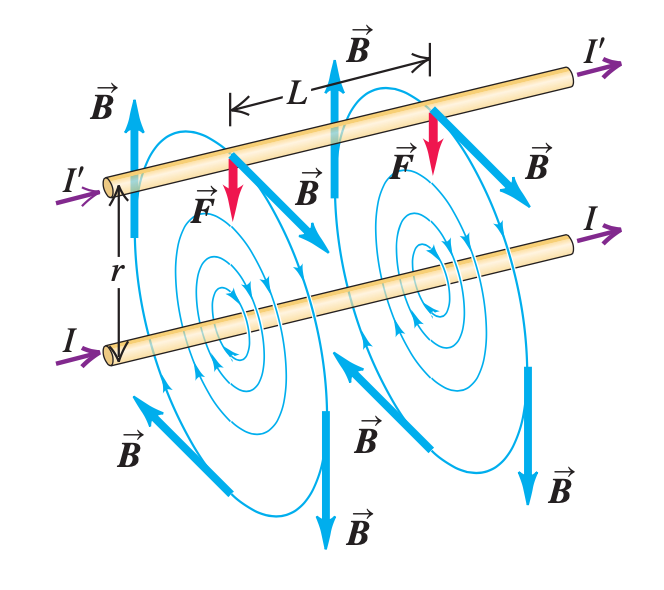
\includegraphics[scale=0.6]{fig/image2}
\centering
\end{figure}
De acuerdo con la ecuación \ref{28.9}, el conductor inferior produce un campo $\vec{B}$ que, en la posición del conductor de arriba, tiene una magnitud $$B=\frac{\mu_0I}{2\pi r}$$ De ecuación (27.19) la fuerza que ejerce este campo sobre una longitud $L$ del conductor superior es $\vec{F}=I' \vec{L}\times\vec{B}$,  donde el vector $\vec{L}$ está en dirección de la corriente $I'$ y tiene magnitud $L$. Como $\vec{B}$ es perpendicular a la longitud del conductor y, por lo tanto, a $\vec{L}$, la magnitud de esta fuerza es $$F=I'LB=\frac{\mu_oII'L}{2\pi r}$$ Luego, la \textit{fuerza por unidad de longitud}, $F/L$ está dada por
\begin{equation}\label{28.11}\marginnote{Magnitud de la fza. entre dos coductores largos, paralelos y portadores de
corriente}
\boxed{\frac{F}{L}=\frac{\mu_0II'}{2\pi r}}
\end{equation}
La aplicación de la regla de la mano derecha a $\vec{F}=I'\vec{L}\times\vec{B}$ indica que la fuerza sobre el conductor de arriba está dirigida hacia abajo.

\textbf{Observación}:
\begin{enumerate}
\item Dos conductores paralelos que transportan corrientes en el mismo sentido se atraen uno al otro.
\item Dos conductores paralelos que transportan corrientes en sentido opuestos se repelen entre sí.
\end{enumerate}
\section{Campo magnético de una espira circular de corriente}
\begin{figure}[h]\label{fig3}
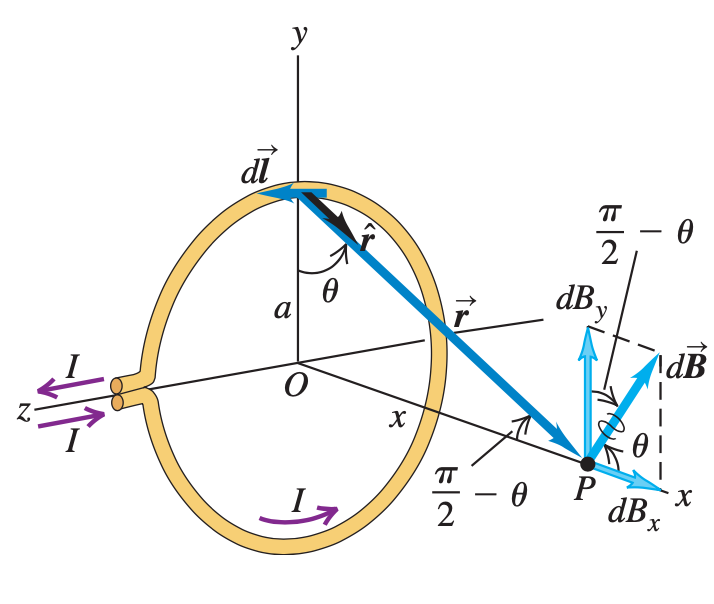
\includegraphics[scale=0.6]{fig/image3}
\centering
\end{figure}
Para encontrar el campo magnético en el punto $P$ sobre el eje de la espira, se usa la ley de Biot y Savart, ecuación \ref{28.5} o \ref{28.6}. De la figura \ref{fig3}, $d\vec{l}$ y $\vec{r}$ son perpendiculares, y la dirección del campo $d\vec{B}$ generado por este elemento $d\vec{l}$ en particular yace sobre el plano $xy$. La magnitud $dB$ del campo debido al elemento $d\vec{l}$ es
\begin{equation}\label{28.15}
\boxed{B_x=\frac{\mu_0Ia^2}{2(x^2+a^2)^{3/2}}}
\end{equation}
Si se cierran los dedos de la mano derecha alrededor de la espira en la dirección de la corriente, el pulgar derecho apunta en la dirección del campo.
\subsection{Campo magnético sobre el eje de una bobina}
Ahora suponga que en vez de una sola espira en la figura \ref{fig3}, se tiene una bobina que consiste en N espiras. Cada espira contribuye por igual al campo, y el total es N veces el campo producido por una sola espira:
\begin{equation}\label{28.16}
B_x=\frac{\mu_0NIa^2}{2(x^2+a^2)^{3/2}}
\end{equation}
En el centro de $N$ espiras circulares la magnitud del campo magnético vale
\begin{equation}\label{28.17}
\boxed{B_x=\frac{\mu_0Ia^2}{2a}}
\end{equation}
Conforme se avanza a lo largo del eje, la magnitud del campo disminuye.
\textbf{Observación}: Las ecuaciones \ref{28.15} y \ref{28.16} son válidas sólo sobre el \textit{eje} de una espira o bobina. No sobre otros puntos.


\section{Ley de Ampere}
\begin{equation}\label{28.20.ampere}\marginnote{Ley de Ampere}\footnote{Sólo válida si las corrientes son estables y si no están presentes materiales magnéticos o campos eléctricos que varíen con el tiempo.}
\boxed{\oint\vec{B}\cdot d\vec{l}=\mu_0I_{enc}}
\end{equation}
Hay una regla simple para determinar el signo de la corriente; Doble los dedos de su mano derecha alrededor de la trayectoria de integración en la dirección de esta última, es decir, la dirección que usa para evaluar $\oint\vec{B}\cdot d\vec{l}$. En esas condiciones, su pulgar derecho indica la dirección de la corriente positiva. Las corrientes que pasan a través de la trayectoria de integración en esta dirección son positivas; aquéllas en dirección opuesta son negativas. La ecuación \ref{28.20.ampere} de hecho es válida para conductores y trayectorias de \textbf{cualquier} forma.

\textbf{Observación}: Si $\oint\vec{B}\cdot d\vec{l}=0$, no necesariamente significa que $\vec{B}=0$
\subsection{Campo de un soleoide}
\begin{figure}[h]
\centering
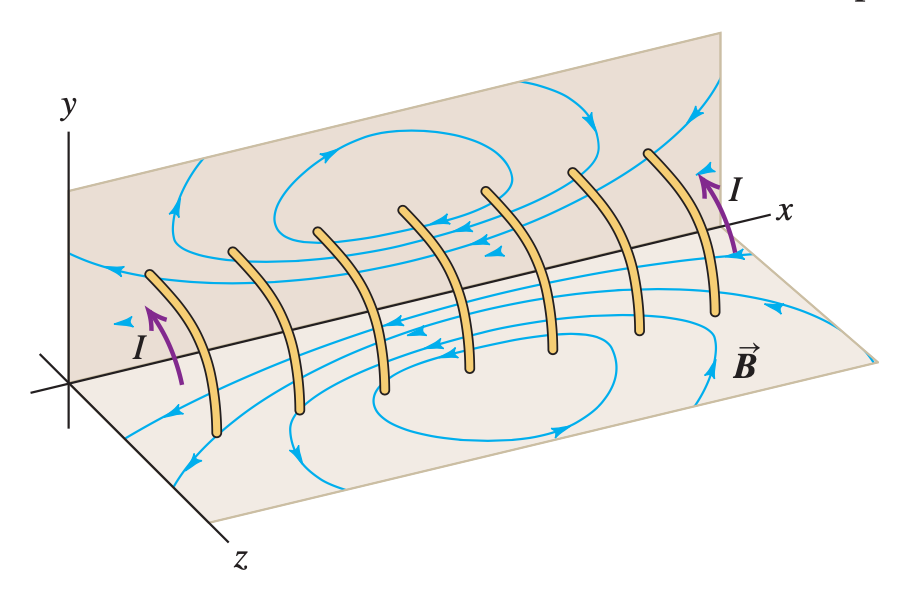
\includegraphics[scale=0.4]{fig/solenoide1}
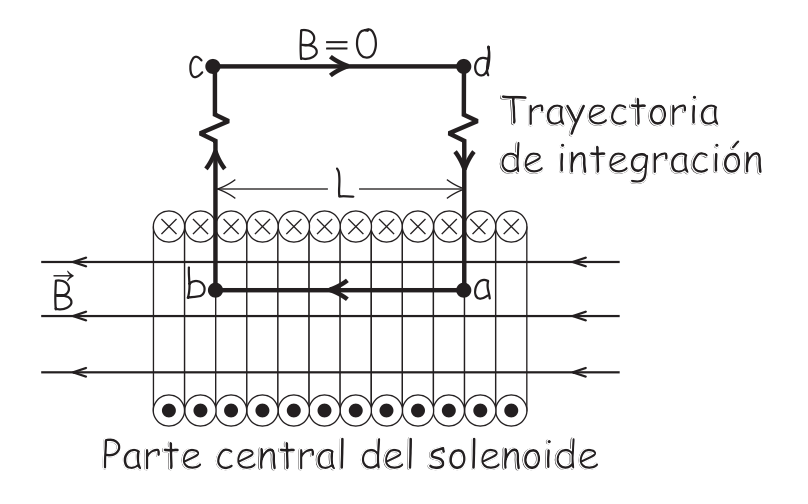
\includegraphics[scale=0.4]{fig/solenoide2}
\end{figure}
Aplicando la ley de Ampere, ecuación \ref{28.20.ampere}, junto con la trayectoria mostrada, se tiene que 
\begin{equation}
B=\mu_0nI
\end{equation}
teniendo en cuenta que $I_{enc}=nLI$.
\subsection{Campo de un solenoide toroidal(toroide)}
\begin{figure}[t]
\centering
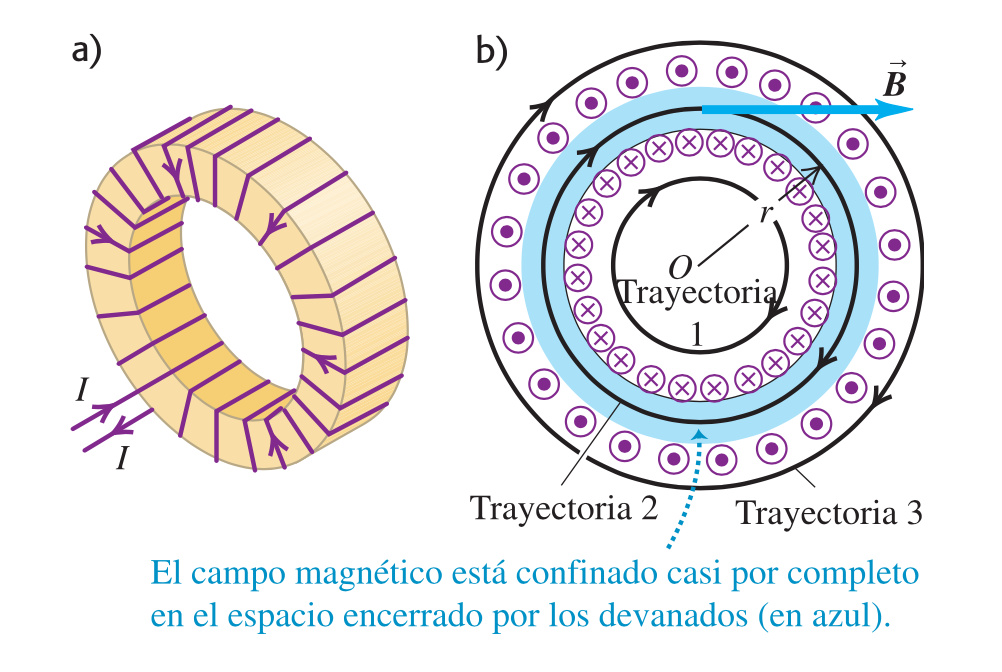
\includegraphics[scale=0.5]{fig/toroide}
\end{figure}
Considerando la trayectoria de integración 1. No hay corriente encerrada, luego $\vec{B}=0$ en cualquier punto de esta trayectoria.

Considernado la trayectoria de integración 3. Cada espira pasa dos veces a través del área limitada por esta trayectoria, llevando corrientes iguales en sentidos opuestos. Luego $I_{enc}=0\rightarrow \vec{B}=0$ en todos los puntos de esta trayectoria.

Considerando la trayectoria 2, un círculo con radio $r$. Se espera que el campo $\vec{B}$ sea tangente a la trayectoria. Por tanto, $\oint\vec{B}\cdot d\vec{l}=2\pi rB$. Despejando $B$
\begin{equation}\label{28.24.toroide}
B=\frac{\mu_0NI}{2\pi r}
\end{equation}
%\end{document}
